\documentclass[10pt]{article}
%%%%%%%%%%%%%%% Define following before importing preamble
\def\Type{LessonCaelan}
\def\TypeNum{Lesson 4}
\def\TypeTitle{Limits and Infinity }
\def\Semester{Fall 2021} %Not Used 
\def\Course{MATH 1190 \& 1210}
\def\Targets{ {\bf\color{RoyalBlue}L2}, {\bf\color{RoyalBlue}L3} }

%%%%%%%%%%%%%%%Preamble must come after above%%%%%%%
\usepackage{preambleDJ}



%%%%%%%%%%%% BEGIN DOCUMENT %%%%%%%%%%%%%%%
%%%%%%%%%%%% BEGIN DOCUMENT %%%%%%%%%%%%%%%
%%%%%%%%%%%% BEGIN DOCUMENT %%%%%%%%%%%%%%%
%%%%%%%%%%%% BEGIN DOCUMENT %%%%%%%%%%%%%%%
%%%%%%%%%%%% BEGIN DOCUMENT %%%%%%%%%%%%%%%

\begin{document}

\pagestyle{otherpages}
\thispagestyle{firstpage}
\vs{.4}

\textbf{Intended Learning Outcomes}
After this lesson, you will be able to 

\begin{itemize}
    \item Identify the form of a limit. (\target{L2})
    \item Identify the method to use to evaluate a limit based on its form. (\target{L2})
    \item Evaluate a limit based on its form. (\target{L2})
\end{itemize}

\vspace{-0.5cm}

\hrulefill
\\
\blue{\bf Rust-Remover Warm-up: Exponent Properties} This exercise helps ``knock the rust off" of some exponent properties that we will be using today.\\
\def\sz{.2}
{\large
\noindent\makebox[\linewidth][s]{$\ds \bullet\, x^{-p}=\frac{1}{x^p} \hs{\sz} \bullet\,\frac{1}{x^{-q}}=\frac{x^q}{1}=x^q \hs{\sz} \bullet\, \frac{x^m}{x^n}=\frac{x^{m-n}}{1}=x^{m-n} \hs{\sz} \bullet\,  \frac{x^m}{x^n}=\frac{1}{x^{n-m}} \hs{\sz} \bullet\,   (x^a)^b=x^{a\cdot b} \hs{\sz} \bullet\,  \sqrt[b]{x}=x^\frac{1}{b}$}
}
\enum{
\item Work together at your tables to re-write each expression with only positive exponents. Note that $e$ is a constant: $e\approx2.71828182846\dots$.
\tasksA{4}{
\task $\ds x^{-4}=\unline{.5}{}{.25}$
\task $\ds \frac{4}{7x^{-6}}=\unline{.5}{}{.25}$
\task  $\ds \frac{10x^{-3}}{x^4}=\unline{.5}{}{.25}$
\task $\ds \frac{3e^{-2x}}{5x^{-4}}=\unline{.5}{}{.25}$
}
\vs{.5}
\item Work together at your tables to re-write each expression using exponent notation. All terms with exponents should be in the numerator (negative exponents are ok).
\tasksA{4}{
\task $\ds \sqrt[4]{x}=\unline{.5}{}{.25}$
\task  $\ds \sqrt[4]{x^3}=\unline{.5}{}{.25}$ 
\task  $\ds \frac{1}{\sqrt[4]{x^3+1}}=\unline{.5}{}{.25}$ 
\task  $\ds \frac{7x^2}{\sqrt{x^3}}=\unline{.5}{}{.25}$ 
}
}
\vs{.5}
{\bf\color{blue}Warm-up}\exercise Four graphs are given below.\\

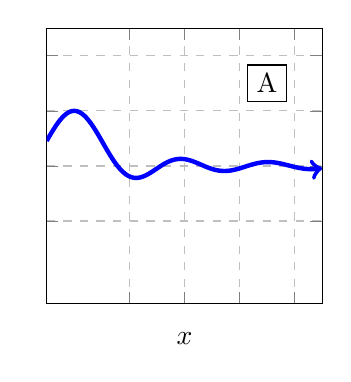
\begin{tikzpicture}[scale=1]
          \begin{axis}[
        %    axis y line = left,
        %    axis x line = bottom,
            xlabel={$x$},
            xtick       = {1,2,3,4},
            xticklabels = {},
            ytick       = {1,2,3,4},
            yticklabels = {},
            samples     = 160,
            domain      = -1:4.5,
            restrict y to domain=-1:4.5,
            xmin = -0.5, xmax = 4.5,
            ymin = -0.5, ymax = 4.5,
            grid=both, grid style=dashed,
            width=2in, height=2in
          ]
          % pieces 1 and 2
          \addplot[domain=-0.5:4.5, blue, ultra thick, ->] {2+sin(4*deg(x))/4/x};
          \node at (3.5,3.5) {\fbox{A}};
        \end{axis}
    \end{tikzpicture}
%
\hfill
%
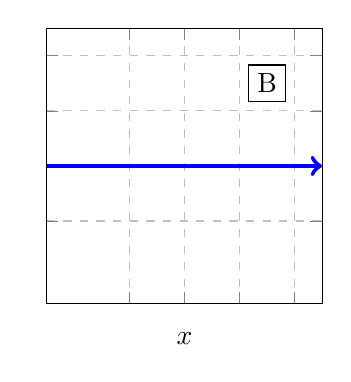
\begin{tikzpicture}[scale=1]
          \begin{axis}[
        %    axis y line = left,
        %    axis x line = bottom,
            xlabel={$x$},
            xtick       = {1,2,3,4},
            xticklabels = {},
            ytick       = {1,2,3,4},
            yticklabels = {},
            samples     = 160,
            domain      = -1:4.5,
            restrict y to domain=-1:4.5,
            xmin = -0.5, xmax = 4.5,
            ymin = -0.5, ymax = 4.5,
            grid=both, grid style=dashed,
            width=2in, height=2in
          ]
          % pieces 1 and 2
          \addplot[domain=-0.5:4.5, blue, ultra thick, ->] {2};
          \node at (3.5,3.5) {\fbox{B}};
        \end{axis}
    \end{tikzpicture}
%
\hfill
%
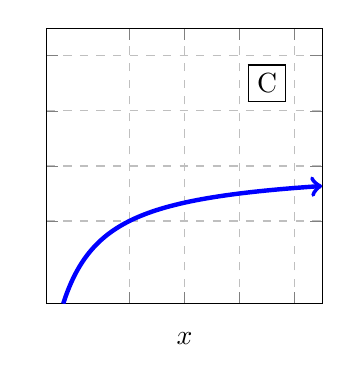
\begin{tikzpicture}[scale=1]
          \begin{axis}[
        %    axis y line = left,
        %    axis x line = bottom,
            xlabel={$x$},
            xtick       = {1,2,3,4},
            xticklabels = {},
            ytick       = {1,2,3,4},
            yticklabels = {},
            samples     = 160,
            domain      = -1:4.5,
            restrict y to domain=-1:4.5,
            xmin = -0.5, xmax = 4.5,
            ymin = -0.5, ymax = 4.5,
            grid=both, grid style=dashed,
            width=2in, height=2in
          ]
          % pieces 1 and 2
          \addplot[domain=-0.2:4.5, blue, ultra thick, ->] {2-2/(x+1)};
          \node at (3.5,3.5) {\fbox{C}};
        \end{axis}
    \end{tikzpicture}
%
\hfill
%
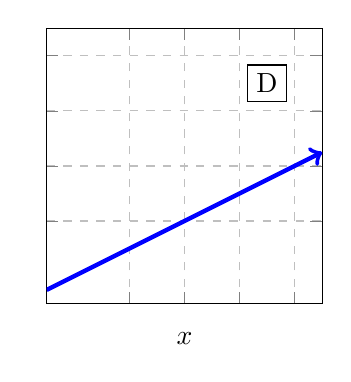
\begin{tikzpicture}[scale=1]
          \begin{axis}[
        %    axis y line = left,
        %    axis x line = bottom,
            xlabel={$x$},
            xtick       = {1,2,3,4},
            xticklabels = {},
            ytick       = {1,2,3,4},
            yticklabels = {},
            samples     = 160,
            domain      = -1:4.5,
            restrict y to domain=-1:4.5,
            xmin = -0.5, xmax = 4.5,
            ymin = -0.5, ymax = 4.5,
            grid=both, grid style=dashed,
            width=2in, height=2in
          ]
          % pieces 1 and 2
          \addplot[domain=-0.5:4.5, blue, ultra thick, ->] {0.5*x};
          \node at (3.5,3.5) {\fbox{D}};
        \end{axis}
    \end{tikzpicture}

For each statement below, decide which of the graphs appears to satisfy the statement. Specify all applicable answers.\\
\begin{enumerate}
\item[(a)] $\displaystyle\lim_{x\to\infty}f(x)=2$ \dotfill \unline{1.5}{}{.25}\\
\item[(b)] $\displaystyle\lim_{x\to\infty}f(x)$ exists \dotfill \unline{1.5}{}{.25}\\
\item[(c)] $\displaystyle\lim_{x\to\infty}f(x)$ DNE\dotfill  \unline{1.5}{}{.25}\\
\end{enumerate}
\newpage
\mpageT{.75}{.25}[\hs{.1}]{
\minil {\it Functions with Infinite Limits at Infinity}\\
{\em Exponentials \hfill Power Functions \hfill Logarithms}
}{
    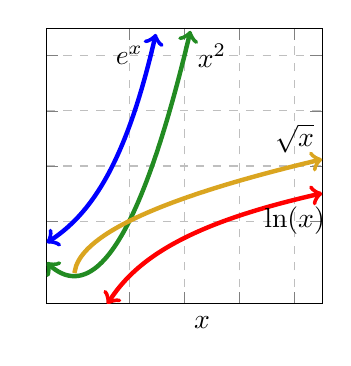
\begin{tikzpicture}[scale=1]
          \begin{axis}[
        %    axis y line = left,
        %    axis x line = bottom,
            xlabel={$x$},
            xtick       = {1,2,3,4},
            xticklabels = {},
            ytick       = {1,2,3,4},
            yticklabels = {},
            xlabel style={anchor=west},
            ylabel style={anchor=south},
            samples     = 160,
            domain      = -1:4.5,
            restrict y to domain=-1:4.5,
            xmin = -0.5, xmax = 4.5,
            ymin = -0.5, ymax = 4.5,
            grid=both, grid style=dashed,
            width=2in, height=2in
          ]
          % pieces 1 and 2
          \addplot[domain=-0.5:4.5, blue, ultra thick, <->] {e^x};
          \node at (2.5,4) {$x^2$};
          \addplot[domain=-0.5:4.5, ForestGreen, ultra thick, <->] {x^2};
          \node at (1,4) {$e^x$};
          \addplot[domain=-0.5:4.5, Goldenrod, ultra thick, ->] {x^(1/2)};
          \node at (4,2.5) {$\sqrt{x}$};
          \addplot[domain=0.6:4.5, red, ultra thick, <->] {ln(x)};
          \node at (4,1) {$\ln(x)$};
        \end{axis}
    \end{tikzpicture}
}

\lform   \blue{  \bf$\dfrac{c}{\infty}$} 
\exercise{\target{L2}} Use your knowledge of numbers and fractions to select an appropriate answer choice for the question below. If you aren't sure how to answer, then try to come up with some fractions in which the given situations occur to help you to form a guess.\\

When the {\it denominator} of a fraction grows ever larger without bound - all other things held constant - the value of the fraction...\\
\mpageT{.5}{.5}{
    \begin{enumerate}
    \item[A.] approaches $0$.
    \item[B.] becomes larger.
    \item[C.] becomes larger without bound.
    \item[D.] could become larger, approach $0$, or anything in between based on the given information.
    \end{enumerate}
    }{
    }
    


\example{\color{RoyalBlue}L2} Find the following limits using forms:\\

$\displaystyle\lim_{x\to\infty} \frac{1}{x^5}=$ \unline{.5}{}{.25}
\hfill 
$\displaystyle\lim_{x\to\infty} \frac{10}{\log_4(x)+\sqrt{x-4}}=$ \unline{.5}{}{.25}
\hfill $\displaystyle\lim_{x\to\infty} 6e^{-x}=$ \unline{.5}{}{.25}
\hfill

\vfill

\exercise{\color{RoyalBlue}L2} Find the following limits using forms. (Practice showing your work, even if you know the answer!)\\

$\displaystyle\lim_{x\to\infty} 5x^{-3}=$ \unline{.5}{}{.25}
\hfill 
$\displaystyle\lim_{x\to\infty} -\frac{1}{e^x+x^{1000}}=$ \unline{.5}{}{.25}
\hfill $\displaystyle\lim_{x\to\infty} \frac{e^{-x}}{x^2} =$ \unline{.5}{}{.25}
\hfill
\vfill
\newpage


\lform  \blue{\bf $\dfrac{\infty}{c}$ }


\exercise{\target{L2}} Use your knowledge of numbers and fractions to select an appropriate answer choice for the question below. If you aren't sure how to answer, then try to come up with some fractions in which the given situations occur to help you to form a guess.\\

When the {\it numerator} of a fraction grows ever larger without bound - all other things held constant - the value of the fraction...\\
\mpageT{.5}{.5}{
    \begin{enumerate}
    \item[A.] approaches $0$.
    \item[B.] becomes larger.
    \item[C.] becomes larger without bound.
    \item[D.] could become larger, approach $0$, or anything in between based on the given information.
    \end{enumerate}
}{
}\vs{.1}\\ 
\example{\target{L2}} Find the following limits using forms:\\

$\displaystyle\lim_{x\to\infty} \frac{e^x+1}{2}=$ \unline{.5}{}{.25}
\hfill 
$\displaystyle\lim_{x\to\infty} \frac{-2x^2}{3\sqrt[4]{x}}=$ \unline{.5}{}{.25}
\hfill 
$\displaystyle\lim_{x\to\infty} \frac{1-\ln(x)}{-3}=$ \unline{.5}{}{.25} 
\hfill

\vfill

\exercise{\target{L2}} Find the following limits using forms. (Practice showing your work, even if you know the answer!)\\

$\displaystyle\lim_{x\to\infty} -\frac{\sqrt{x}}{5}=$ \unline{.5}{}{.25}
\hfill 
$\displaystyle\lim_{x\to\infty} \frac{x^5}{2x}=$ \unline{.5}{}{.25}
\hfill 
$\displaystyle\lim_{x\to\infty} \frac{1}{2e^{-x}}=$ \unline{.5}{}{.25}
\hfill

\vfill

%%%%%%%%%
\newpage%
%%%%%%%%%

%$\left({\it \text{\bf \blue{Form} }\dfrac{\infty}{\infty}}\right)$
\lform  \blue{\bf $\dfrac{\infty}{\infty}$}


\exercise{\target{L2}} Use your knowledge of numbers and fractions to select an appropriate answer choice for the question below. If you aren't sure how to answer, then try to come up with some fractions in which the given situations occur to help you to form a guess.\\

When both the {\it numerator and denominator} grow ever larger without bound, the value of the fraction...\\
\mpageT{.5}{.5}{
    \begin{enumerate}
    \item[A.] approaches $0$.
    \item[B.] becomes larger.
    \item[C.] becomes larger without bound.
    \item[D.] could become larger, approach $0$, or anything in between based on the given information.
    \end{enumerate}
}{
}\\
%%%

\mpageT{.75}{.25}[\hs{.1}]{
\minil{\it Dominance Hierarchy in Limits at Infinty, i.e. ``Pecking Order"}\\
{\em Exponentials \hfill Power Functions \hfill Logarithms}
}{
    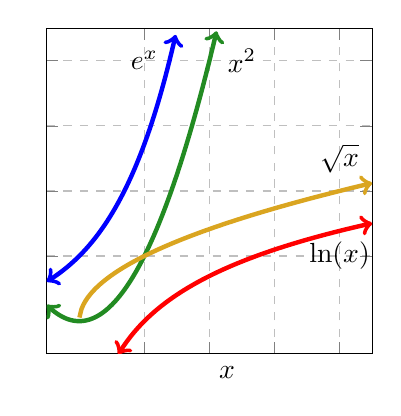
\begin{tikzpicture}[scale=1]
          \begin{axis}[
        %    axis y line = left,
        %    axis x line = bottom,
            xlabel={$x$},
            xtick       = {1,2,3,4},
            xticklabels = {},
            ytick       = {1,2,3,4},
            yticklabels = {},
            xlabel style={anchor=west},
            ylabel style={anchor=south},
            samples     = 160,
            domain      = -1:4.5,
            restrict y to domain=-1:4.5,
            xmin = -0.5, xmax = 4.5,
            ymin = -0.5, ymax = 4.5,
            grid=both, grid style=dashed,
            width=2.25in, height=2.25in
          ]
          % pieces 1 and 2
          \addplot[domain=-0.5:4.5, blue, ultra thick, <->] {e^x};
          \node at (2.5,4) {$x^2$};
          \addplot[domain=-0.5:4.5, ForestGreen, ultra thick, <->] {x^2};
          \node at (1,4) {$e^x$};
          \addplot[domain=-0.5:4.5, Goldenrod, ultra thick, ->] {x^(1/2)};
          \node at (4,2.5) {$\sqrt{x}$};
          \addplot[domain=0.6:4.5, red, ultra thick, <->] {ln(x)};
          \node at (4,1) {$\ln(x)$};
        \end{axis}
    \end{tikzpicture}
}
{\em Key Idea for Form $\dfrac{\infty}{\infty}$}
\vs{1}\\
\example{\target{L2}} Find the following limits using forms:\\

$\displaystyle\lim_{x\to\infty} \frac{\log_2(x)}{x^3+4x-1}=$ \unline{.5}{}{.25}
\hfill 
$\displaystyle\lim_{x\to\infty} \frac{4^x+\ln(x)}{1-\sqrt[3]{x}}=$ \unline{.5}{}{.25} 
\hfill 
$\displaystyle\lim_{x\to\infty} \frac{\log_2(x)-\sqrt{x}}{2\sqrt{x+5}-4}=$ \unline{.5}{}{.25}
\hfill\,
\vs{1.5}~\\

\newpage
\exercise{\target{L2}} Find the following limits using forms. (Practice showing your work, even if you  know the answer!)\\[0.2in]

$\displaystyle\lim_{x\to\infty} \frac{7^x-x}{x^7}=$ \unline{.5}{}{.25}
\hfill 
$\displaystyle\lim_{x\to\infty} \frac{\sqrt{x+1}}{4-x-\ln(x)}=$ \unline{.5}{}{.25}
\hfill 
$\displaystyle\lim_{x\to\infty} \frac{\sqrt{x^2+1}}{4-3x-\ln(x)}=$ \unline{.5}{}{.25}
\hfill\,
\vs{1.5}~\\

$\displaystyle\lim_{x\to\infty} \frac{1000-x^{1000}}{x^e-e^x}=$ \unline{.5}{}{.25}
\hfill 
$\displaystyle\lim_{x\to\infty} \frac{5e^{2x}+3e^x+1}{e^{2x}-5e^x+6}=$ \unline{.5}{}{.25} 
\hfill
%$\displaystyle\lim_{x\to\infty} \frac{x^5 +3x+\ln(x)}{2x+3}=$ \unline{.5}{}{.25} 
\vs{2}\\
\blue{\bf Summary of Limit Form   $\dfrac{\infty}{\infty}$}
After choosing dominant terms in numerator and denominator....
\itemI{
\item $\ds \frac{\text{much faster}}{\text{slower}}\to$
\vs{.75}
\item $\ds \frac{\text{slower}}{\text{much faster}}\to$
\vs{.75}
\item $\ds \frac{\text{about the same}}{\text{about the same}}\to$
}

%%%%%%%%%

%%%%%%%%%
\newpage
%$\left({\it \text{\bf \blue{Form} }\dfrac{c}{0}}\right)$
\lform $\blue{\bf \dfrac{c}{0}}$



\exercise{\target{L2}}  Use your knowledge of numbers and fractions to select an appropriate answer choice for the question below. If you aren't sure how to answer, then try to come up with some fractions in which the given situations occur to help you to form a guess.\\

When the {\it denominator} of a fraction grows ever smaller - approaching $0$ - with all other things held constant, the value of the fraction...\\
\mpageT{.5}{.5}{
    \begin{enumerate}
    \item[A.] approaches $0$.
    \item[B.] becomes larger.
    \item[C.] becomes larger without bound.
    \item[D.] could become larger, approach $0$, or anything in between based on the given information.
    \end{enumerate}
}{
}
\vs{.1}\\
\minil What can be said about a limit if we know its form resembles $\dfrac{c}{0}$? Specify the various cases as well as what you can conclude in each of those cases.\\
\mpageT{.5}{.5}{
\mbox{}
}{
\begin{flushright}
\begin{tabular}{|>{\columncolor{lightgray}}c|c|c|}  \hline
\rowcolor{lightgray}&\hs{1}&\hs{1}\\
\rowcolor{lightgray}$\ds \to\frac{c}{0}$&Num $\to (+)$&Num $\to (-)$\\ 
\rowcolor{lightgray}&& \\ \hline
&&\\
Denom $\to 0^+$ && \\ 
&&\\
&& \\ \hline
&&\\
Denom $\to 0^-$&&\\
&&\\
&&\\ \hline
\end{tabular}
\end{flushright}
}
\vfill
\vfill

\newpage

\example{\target{L2}} Find the following limits using forms:
	\enumA{
\mpageT{.5}{.5}{
	\item $\displaystyle\lim_{x\to1^{-}} \frac{\sqrt{x}+1}{x-1}=$\unline{1}{}{.25}
	}{
	\item $\displaystyle\lim_{x\to3} \frac{x^2-2x}{3-x}=$\unline{1}{}{.25}
	}
	\vs{3.5}\\
\exercise{\color{RoyalBlue}L2} Find the following limits using forms:\\
\mpageT{.5}{.5}{
	\item $\displaystyle\lim_{x\to 0^+}\frac{1+x}{x^2}=$\unline{1}{}{.25}
}{
\item $\displaystyle\lim_{x\to 5}\frac{1+x}{x^2-25}=$\unline{1}{}{.25}
}

	}

%%%%%%%%%
\newpage%
%%%%%%%%%

{\bf\color{blue}Extra Practice 1.}\reversemarginpar\marginnote{\fbox{\bf\color{RoyalBlue}L2}} Find the following limits using either forms or continuity.\\

\begin{tabular}{ p{3.25in} | p{3.25in} }
%
$\displaystyle\lim_{x\to1^+} (1-x)^{-3} $ & $\displaystyle\lim_{x\to\infty} (1-x)^{-3}$\\[2in]
%
\hline
%
$\displaystyle\lim_{x\to\infty} \frac{x^2-4x-\sqrt{x}}{1-\sqrt[3]{x^2-2x}}$ & $\displaystyle\lim_{x\to4} \frac{x^2-4x-\sqrt{x}}{1-\sqrt[3]{x^2-2x}}$\\[2in]
%
\hline
%
$\displaystyle\lim_{x\to\infty} \dfrac{\sqrt[3]{x^7+1}-x}{\ln(x)+x^2} $ & $\displaystyle\lim_{x\to\infty} \dfrac{\ln(x)+x^2}{\sqrt[3]{x^7+1}-x}$\\[2in]
%
\hline
%
$\displaystyle\lim_{x\to\infty} \frac{e^x+e^{-x}}{e^x-e^{-x}} $ & $\displaystyle\lim_{x\to0^-} \frac{e^x+e^{-x}}{e^x-e^{-x}} $\\[2in]
%
\end{tabular}

\end{document}
